% Options for packages loaded elsewhere
\PassOptionsToPackage{unicode}{hyperref}
\PassOptionsToPackage{hyphens}{url}
%
\documentclass[
  a4paper,
  twoside, 11pt]{article}
\usepackage{amsmath,amssymb}
\usepackage{lmodern}
\usepackage{ifxetex,ifluatex}
\ifnum 0\ifxetex 1\fi\ifluatex 1\fi=0 % if pdftex
  \usepackage[T1]{fontenc}
  \usepackage[utf8]{inputenc}
  \usepackage{textcomp} % provide euro and other symbols
\else % if luatex or xetex
  \usepackage{unicode-math}
  \defaultfontfeatures{Scale=MatchLowercase}
  \defaultfontfeatures[\rmfamily]{Ligatures=TeX,Scale=1}
\fi
% Use upquote if available, for straight quotes in verbatim environments
\IfFileExists{upquote.sty}{\usepackage{upquote}}{}
\IfFileExists{microtype.sty}{% use microtype if available
  \usepackage[]{microtype}
  \UseMicrotypeSet[protrusion]{basicmath} % disable protrusion for tt fonts
}{}
\makeatletter
\@ifundefined{KOMAClassName}{% if non-KOMA class
  \IfFileExists{parskip.sty}{%
    \usepackage{parskip}
  }{% else
    \setlength{\parindent}{0pt}
    \setlength{\parskip}{6pt plus 2pt minus 1pt}}
}{% if KOMA class
  \KOMAoptions{parskip=half}}
\makeatother
\usepackage{xcolor}
\IfFileExists{xurl.sty}{\usepackage{xurl}}{} % add URL line breaks if available
\IfFileExists{bookmark.sty}{\usepackage{bookmark}}{\usepackage{hyperref}}
\hypersetup{
  hidelinks,
  pdfcreator={LaTeX via pandoc}}
\urlstyle{same} % disable monospaced font for URLs
\usepackage[top=2cm, outer=3.5cm, bottom=3cm, inner=3.5cm]{geometry}
\usepackage{longtable,booktabs,array}
\usepackage{calc} % for calculating minipage widths
% Correct order of tables after \paragraph or \subparagraph
\usepackage{etoolbox}
\makeatletter
\patchcmd\longtable{\par}{\if@noskipsec\mbox{}\fi\par}{}{}
\makeatother
% Allow footnotes in longtable head/foot
\IfFileExists{footnotehyper.sty}{\usepackage{footnotehyper}}{\usepackage{footnote}}
\makesavenoteenv{longtable}
\usepackage{graphicx}
\makeatletter
\def\maxwidth{\ifdim\Gin@nat@width>\linewidth\linewidth\else\Gin@nat@width\fi}
\def\maxheight{\ifdim\Gin@nat@height>\textheight\textheight\else\Gin@nat@height\fi}
\makeatother
% Scale images if necessary, so that they will not overflow the page
% margins by default, and it is still possible to overwrite the defaults
% using explicit options in \includegraphics[width, height, ...]{}
\setkeys{Gin}{width=\maxwidth,height=\maxheight,keepaspectratio}
% Set default figure placement to htbp
\makeatletter
\def\fps@figure{htbp}
\makeatother
\setlength{\emergencystretch}{3em} % prevent overfull lines
\providecommand{\tightlist}{%
  \setlength{\itemsep}{0pt}\setlength{\parskip}{0pt}}
\setcounter{secnumdepth}{-\maxdimen} % remove section numbering
% change line spacing
\usepackage[onehalfspacing]{setspace}

% change font to Helvetica for titles and Garamond for body text
\usepackage[scaled]{helvet}
% \usepackage{garamondx}
\usepackage[T1]{fontenc}
% \renewcommand\familydefault{\sfdefault}

% allow coloured text and boxes
\usepackage{xcolor}
\definecolor{uclyellow}{HTML}{F6BE00}

% change section titles
\usepackage{titlesec}
\titleformat{\section}{\bigskip\raggedright\LARGE\sffamily}{\thesection}{0.5em}{}[\titlerule]

% allow absolute positioning of blocks on title page
\usepackage[absolute]{textpos}
\setlength{\TPHorizModule}{1cm}
\setlength{\TPVertModule}{\TPHorizModule}
\textblockorigin{0cm}{0cm}

% override default placement of figures by pandoc, which is different from the 
% latex default -- this code works in conjunction with the knitr option 
% `fig.pos = 'tbp'`
\usepackage{float}

% move captions above figures
% \usepackage{floatrow}
% \floatsetup[figure]{capposition=top}

% make tables prettier
\usepackage{booktabs}

% prevent widows and orphans
% \widowpenalty 10000
% \clubpenalty 10000

% setup PDF options
\hypersetup{
    colorlinks=true,
    linkcolor=blue,
    filecolor=blue,      
    urlcolor=blue,
    pdftitle={Stop and search in London},
    bookmarks=true
}
\usepackage[onehalfspacing]{setspace}
\usepackage[scaled]{helvet}
\usepackage[T1]{fontenc}
\usepackage{xcolor}
\definecolor{uclyellow}{HTML}{F6BE00}
\usepackage{titlesec}
\titleformat{\section}{\bigskip\raggedright\LARGE\sffamily}{\thesection}{0.5em}{}[\titlerule]
\usepackage[absolute]{textpos}
\setlength{\TPHorizModule}{1cm}
\setlength{\TPVertModule}{\TPHorizModule}
\textblockorigin{0cm}{0cm}
\usepackage{float}
\usepackage{booktabs}
\hypersetup{colorlinks=true, linkcolor=blue, filecolor=blue, urlcolor=blue, pdftitle={Stop and search in London}, bookmarks=true}
\ifluatex
  \usepackage{selnolig}  % disable illegal ligatures
\fi

\author{}
\date{\vspace{-2.5em}}

\begin{document}

\frenchspacing

\raggedright

\raggedbottom

\begin{textblock*}{21cm}(0mm, 0mm)
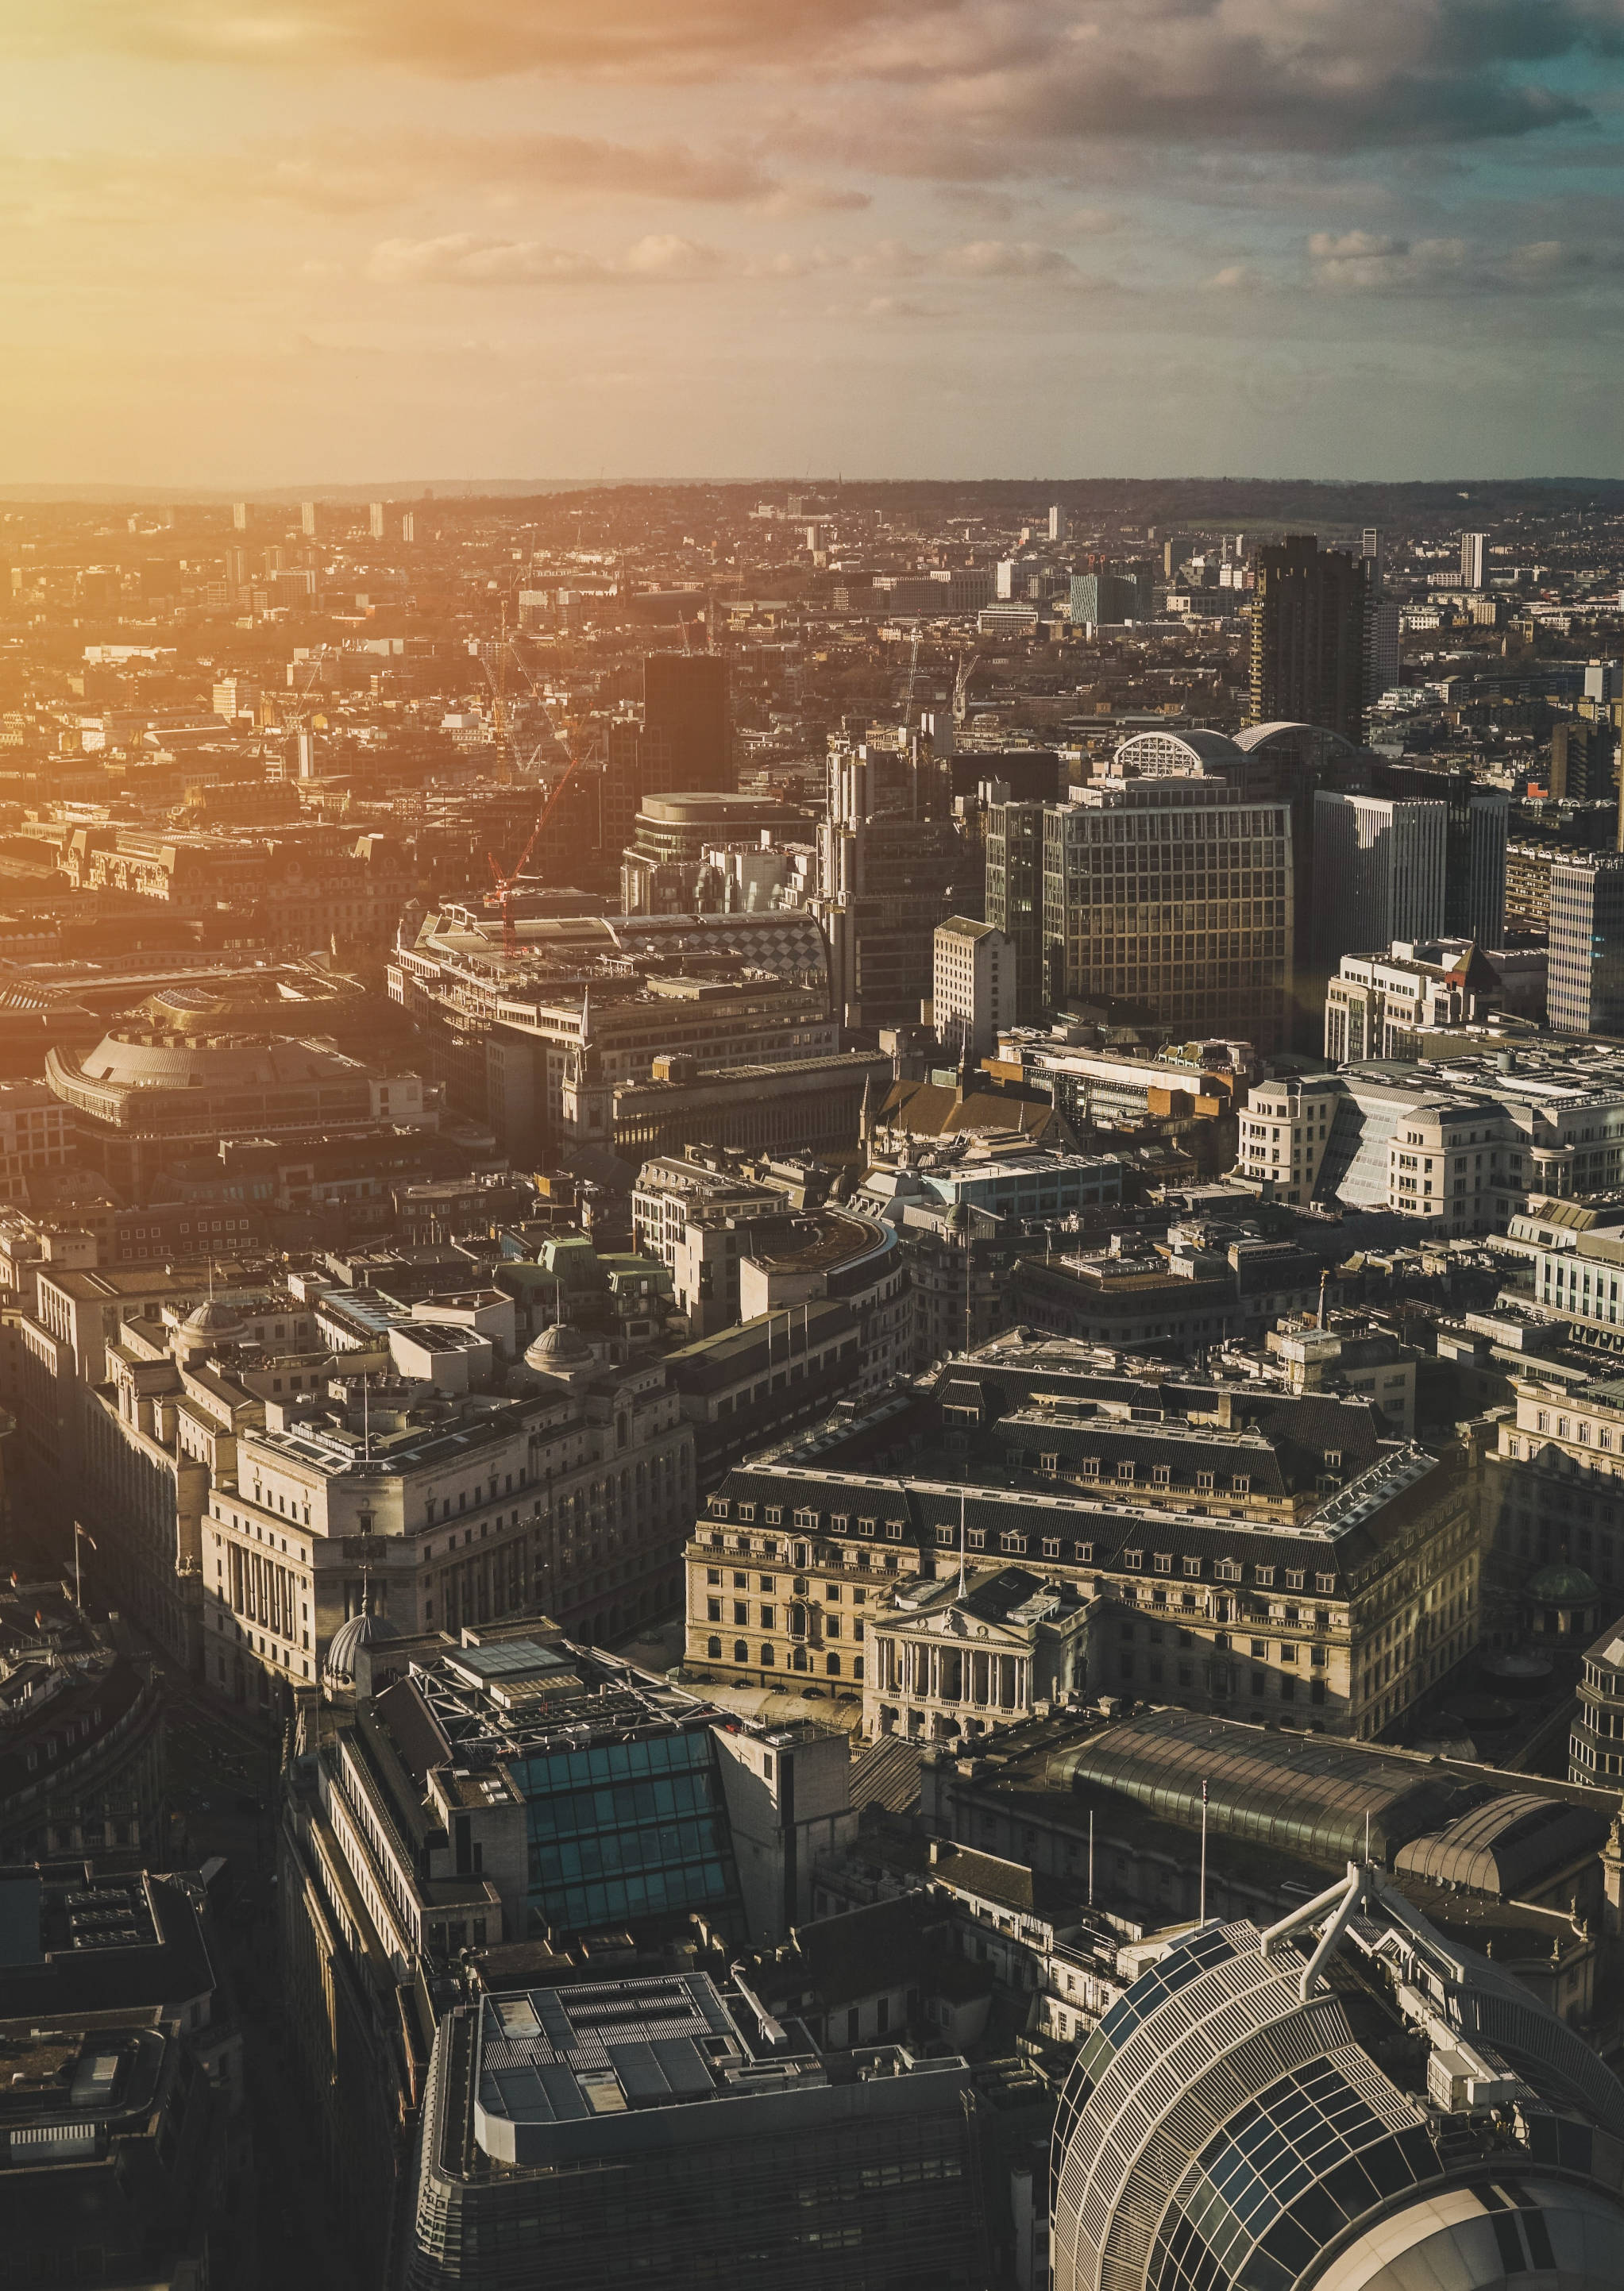
\includegraphics[width=21cm,height=29.7cm]{cover_image_2020_q4.jpg}
\end{textblock*}

\begin{textblock*}{21cm}(0mm, 0mm)

\includegraphics[width=21cm]{ucl-banner-port-yellow-rgb-lg.png}
\end{textblock*}

\begin{textblock*}{21cm}(1cm,1cm)
\textbf{\sffamily INSTITUTE FOR GLOBAL CITY POLICING}
\end{textblock*}

\begin{textblock*}{18cm}(3cm, 13.66cm)
\raggedright \sffamily
\begin{singlespace}
\colorbox{white}{\hspace{1cm}\parbox[c][5.9cm]{16cm}{
{\fontsize{40}{32}\selectfont \bfseries 
\mbox{Stop and search}\\\mbox{in North West BCU}
\vspace{6pt}}

{\fontsize{36}{30}\selectfont \mbox{January to December 2020} }

}\hspace{1cm}}
\end{singlespace}
\end{textblock*}

\begin{textblock*}{11.43cm}(0cm, 24.13cm)
\colorbox{uclyellow}{\parbox[c][2.63cm]{\textwidth}{
\centering \bfseries \sffamily \fontsize{16}{16}\selectfont 
Dr Matt Ashby\ \ |\ \ July 2021
}}
\end{textblock*}

~

\thispagestyle{empty}
\newpage

\hypertarget{main-points}{%
\section{Main points}\label{main-points}}

\textbf{\sffamily Police in North West BCU (Barnet, Brent, and Harrow boroughs) stopped and searched 19,963 people and vehicles in the 12~months from January to December 2020. The number of searches has generally increased over the past two years.}

\textbf{\sffamily 69\% of searches in that period were for drugs, with 77\% of all searches resulting in no further action.}

\textbf{\sffamily Searches are heavily concentrated in some areas -- half of all searches occurred in 11\% of neighbourhoods.}

\hypertarget{introduction}{%
\section{Introduction}\label{introduction}}

Stop and search is a legal power that allows police officers to search people to find out if they are carrying prohibited items such as drugs, weapons or stolen goods. Stop and search means officers can confirm if a person is or is not in possession of contraband without arresting them and taking them to a police station, but it is also a source of tension between police and communities. \href{https://whatworks.college.police.uk/Research/Documents/SS_and_crime_report.pdf}{A review by the College of Policing} found little relationship between how many searches police do and how much crime occurs, but \href{https://www.met.police.uk/advice/advice-and-information/st-s/stop-and-search/why-we-use-stop-and-search/}{police insist stop and search helps them fight crime}. This report summarises how police used stop and search powers in the North West Basic Command Unit (the London boroughs of Barnet, Brent, and Harrow) from January to December 2020.



\begin{figure}[h]

{\centering 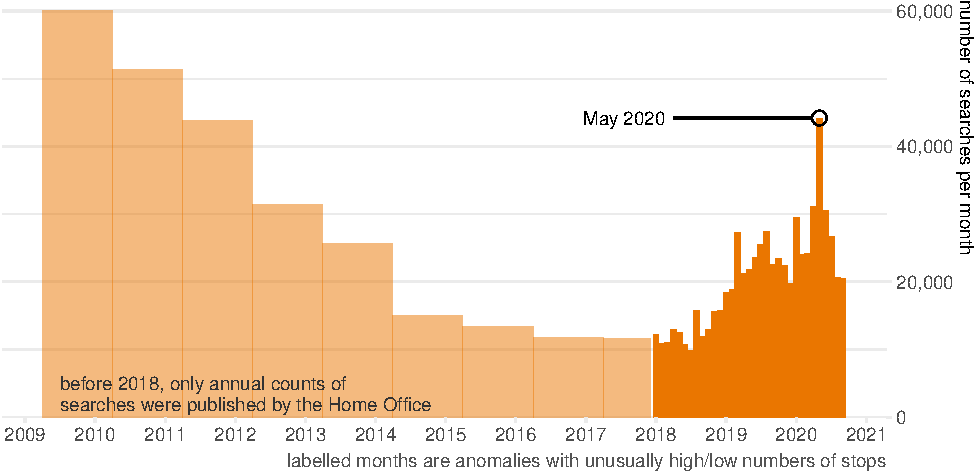
\includegraphics{2020-Q4-bcu_files/figure-latex/chart-trend-overall-1} 

}

\caption{Number of stop-and-searches in North West BCU, January 2018 to December 2020}\label{fig:chart-trend-overall}
\end{figure}

\textbf{Between January and December 2020, police officers in North West BCU carried out 19,963 stop-and-searches}, or about 384 per week -- the lowest rate of searches per 1,000 residents of any the 12 Metropolitan Police BCUs. Of those, 99\% were conducted by the Metropolitan Police and 1\% by British Transport Police. Across both forces, 66\% of stops were of pedestrians, 32\% of people in vehicles and 2\% of only vehicles.

The number of searches carried out in January to December 2020 was \textbf{a year-on-year increase of 38\%} (Figure \ref{fig:chart-trend-overall}) compared to an increase of 20\% across London as a whole.

\hypertarget{what-items-are-people-searched-for}{%
\section{What items are people searched for?}\label{what-items-are-people-searched-for}}



\begin{figure}[h]

{\centering 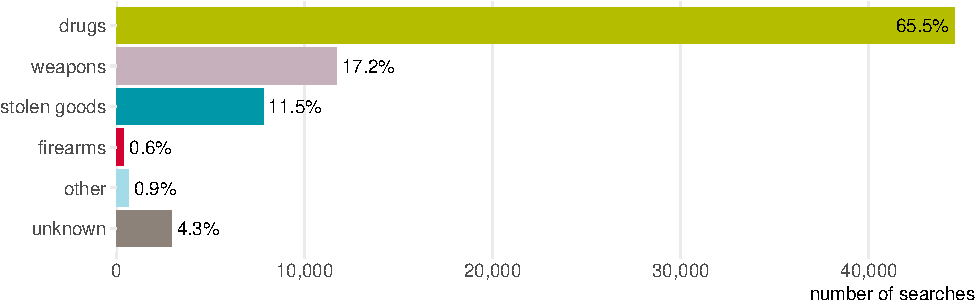
\includegraphics{2020-Q4-bcu_files/figure-latex/chart-search-types-1} 

}

\caption{Searches by type of object being searched for, January to December 2020}\label{fig:chart-search-types}
\end{figure}

Police officers are empowered to search people for different items -- including drugs, items to use in theft or criminal damage, stolen goods, weapons and even some fireworks -- under different acts of parliament. Although police emphasise that stop and search ``\href{https://www.met.police.uk/police-forces/metropolitan-police/areas/about-us/about-the-met/stop-and-search/}{protects Londoners by taking weapons off the streets}'', only about one in six searches in North West BCU between January and December 2020 were for weapons -- \textbf{69\% of searches were for drugs} (Figure \ref{fig:chart-search-types}). North West BCU had the second highest proportion of searches for drugs and the second highest proportion of searches for firearms of the 12 Metropolitan Police BCUs.



\begin{figure}[h]

{\centering 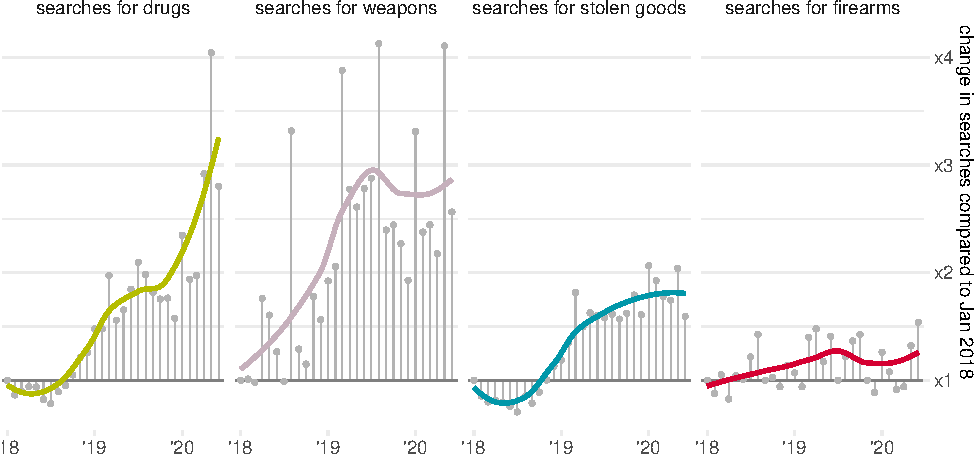
\includegraphics{2020-Q4-bcu_files/figure-latex/chart-search-types-change-1} 

}

\caption{Change in number of searches by type, January 2018 to December 2020}\label{fig:chart-search-types-change}
\end{figure}

About 94\% of searches are looking for the four main types of contraband: drugs, firearms, stolen goods and weapons.

Police can search people for weapons using two different legal powers. Searches under \href{https://www.legislation.gov.uk/ukpga/1984/60/section/1}{section 1 of the Police and Criminal Evidence Act 1984} (PACE) require the officer to have ``reasonable grounds for suspecting'' that the person is carrying an offensive weapon or other prohibited item. Conversely, officers can search people under \href{https://www.legislation.gov.uk/ukpga/1994/33/section/60}{section 60 of the Criminal Justice and Public Order Act 1994} (CJPOA) without having any reason to think the person has a weapon, as long as a more-senior officer believes ``incidents involving serious violence may take place'' in the area. These `section 60' searches are particularly controversial because they allow officers to search \emph{anyone} in an area, even if there is no reason to think they have a weapon in their possession. Between January and December 2020, 89\% of weapons searches in North West BCU were based on reasonable suspicion under PACE section 1, with the remaining 11\% (348 searches, or about 7 per week) were conducted without the need for suspicion based on authorisations under CJPOA section 60. Police do not publish any information about authorisations made under section 60 so it is difficult to track any patterns or trends, although section-60 searches are typically higher in August due to the Notting Hill Carnival, which was cancelled in 2020. The proportion of weapon searches in the North West BCU that were conducted without the need for reasonable suspicion was similar to other Metropolitan Police BCUs.



\begin{figure}[h]

{\centering 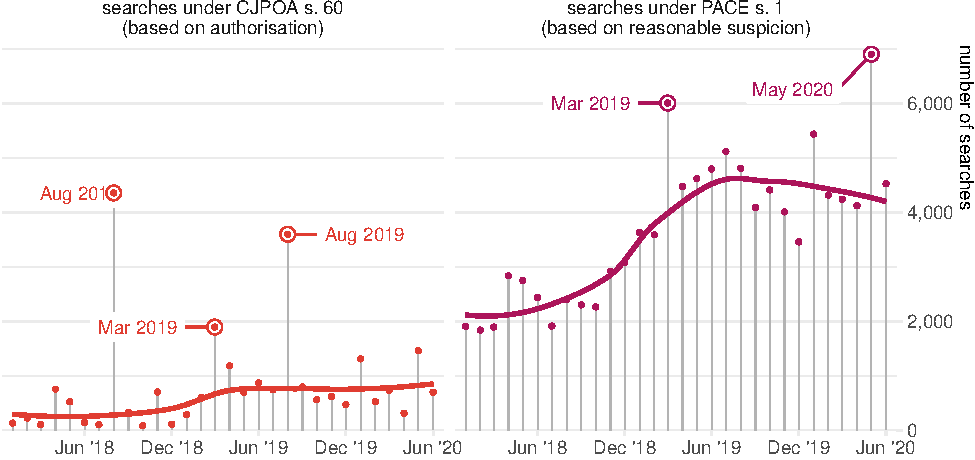
\includegraphics{2020-Q4-bcu_files/figure-latex/chart-trend-weapons-1} 

}

\caption{Change in number of searches for weapons, January 2018 to December 2020}\label{fig:chart-trend-weapons}
\end{figure}

Searches based on reasonable suspicion the person being searched is carrying a weapon have not shown a significant increasing or decreasing trend over the past 12 months (Figure \ref{fig:chart-trend-weapons}). In comparison to that trend, the number of these searches was anomalously high in March 2019.
No-suspicion searches under section 60 have not shown a significant increasing or decreasing trend over the past 12 months, with searches having been anomalously high in August 2018. The number of searches under section 60 is often higher in August because of searches associated with the Notting Hill Carnival, even in other parts of London.

\hypertarget{who-do-police-search}{%
\section{Who do police search?}\label{who-do-police-search}}

Of the 19,645 searches of pedestrians and vehicle occupants in the North West BCU from January to December 2020, \textbf{95\% were searches of men or boys}, compared to 93\% of searches in London as a whole. Of all people searched in the North West BCU, 15\% were aged under 18 -- lower than than the 18\% in London as a whole.

The self-defined ethnicity of the person searched was known for 77\% of searches, of which 38\% of people described themselves as Black/Black British, 31\% as white and 21\% as Asian/Asian British.

\textbf{Search rates vary hugely across different groups}. Of the 50 combinations of sex, age and self-defined ethnicity present in the search data, 14 groups were searched at a higher rate than the rate for the population as a whole (Figure \ref{fig:chart-disparity}). While disparity between ethnic groups has generated much comment, being male and being aged under 35 are more-powerful predictors of a group having a higher search rate than that group being non-white. The reasons for these differences are likely to be complex: many types of offending are concentrated among some groups (particularly young men) as well as in some neighbourhoods, and there are \href{https://www.bbc.co.uk/news/uk-47300343}{longstanding issues of bias and stereotyping among police and in society}. There is also an interaction between factors such as deprivation and the amount of time people spend in public (where almost-all searches occur). There is no way to know from the data analysed here what combination of these factors drives the disparities in search rates.



\begin{figure}[h]

{\centering 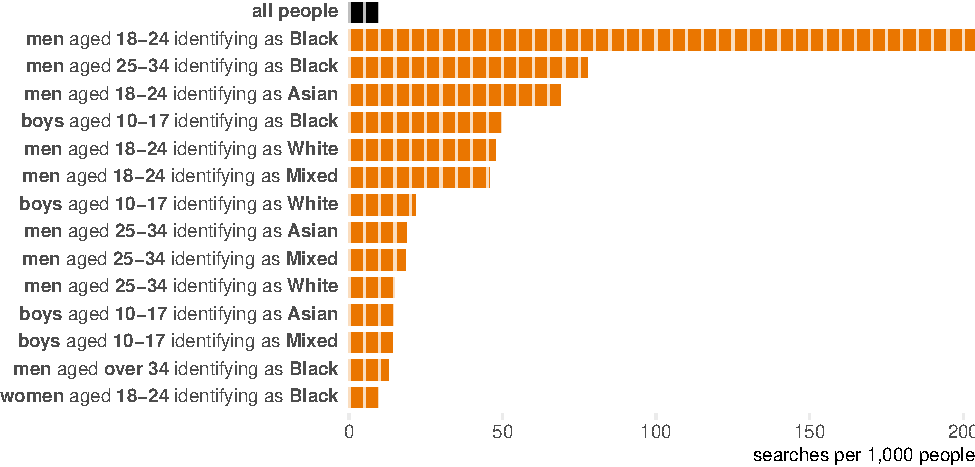
\includegraphics{2020-Q4-bcu_files/figure-latex/chart-disparity-1} 

}

\caption{Search rates for different demographic groups, January to December 2020}\label{fig:chart-disparity}
\end{figure}

In comparison to the population of the North West BCU as a whole, men aged 18-24 identifying as Black (the group with the highest search rate) were on-average 28 times more likely to be stopped and searched. Disparities in search rates also vary according to the type of search. Disparity is highest in searches for weapons (s. 60), for which men aged 18-24 identifying as Black were 32 times more likely to be searched than the population at large. Of the 32 combinations of age, ethnic-group and sex present in the data, the rate of searches in the North West BCU was highest for all five of the main types of search for men aged 18-24 who identified as Black. It is important to note that these disparity ratios only represent \emph{average} search rates for different groups -- they do not reflect the individual experience of everyone in each group. It is likely that a small number of people in each group are being searched repeatedly while others are searched far less often, but since police do not publish data on repeated searches it is difficult to know how this affects overall search rates.

\hypertarget{how-often-do-police-find-items-during-searches}{%
\section{How often do police find items during searches?}\label{how-often-do-police-find-items-during-searches}}

The purpose of stop and search is to ``enable officers to allay or confirm suspicions about individuals without exercising their power of arrest'' (\href{https://www.gov.uk/guidance/police-and-criminal-evidence-act-1984-pace-codes-of-practice}{PACE Code A, paragraph 1.4}). As such, a search that does not find what is being searched for can be considered successful if it prevents an innocent person being arrested and a police officer being taken off the street unnecessarily. There is not necessarily an optimal proportion of searches that should result in the officer finding what they are looking for. Measuring outcomes is also difficult: officers may have legitimate grounds to search a group of people (e.g.~all the occupants in a vehicle believed to contain a firearm) when only one person has contraband in their possession. Nevertheless, all searches are an ``intrusion on the liberty of the person'' (PACE Code A, paragraph 1.2) and high proportions of searches that do not find anything may indicate that searches are not well targeted.

The data released by the Home Office do not specify whether or not the item police were looking for was found during a search. Instead, we can measure whether a search resulted in some formal criminal-justice process such as an arrest. This is not a perfect measure of whether an item was found during a search, because a person might be arrested for some other reason (for example because there was an outstanding warrant for their arrest) or contraband might be found but police deal with it informally. Nevertheless, this is the least-worst measure of search outcomes that is currently available.



\begin{figure}[h]

{\centering 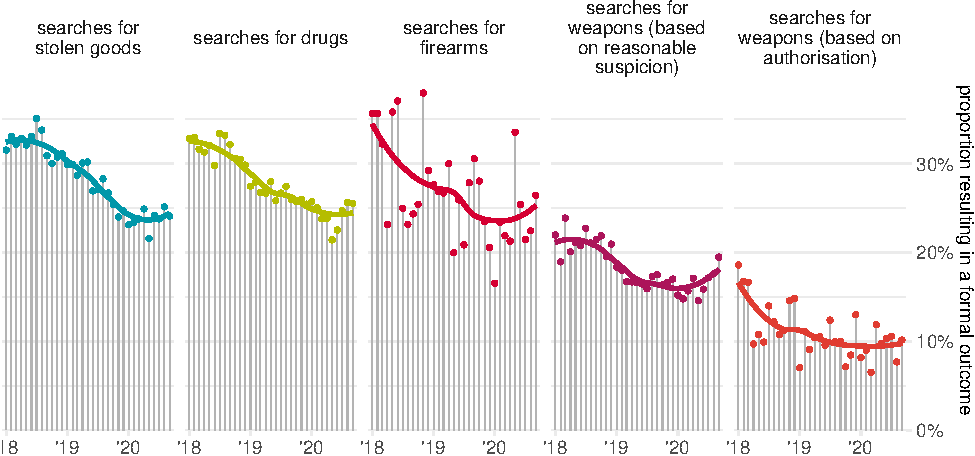
\includegraphics{2020-Q4-bcu_files/figure-latex/chart-results-1} 

}

\caption{Change in proportion of searches with a formal outcome, January 2018 to December 2020}\label{fig:chart-results}
\end{figure}

Overall, about 24\% of searches in the North West BCU between January and December 2020 resulted in a formal criminal-justice outcome (arrest, caution, charged by post, community/local resolution, drugs warning or fixed penalty), while the remaining \textbf{76\% of searches resulted in no further action.} The proportion of stops in the North West BCU with a formal outcome was about the same as the proportion (23\%) in London as a whole. Over the past year, searches for firearms have been most likely to lead to a formal outcome (29\%, slightly higher than the 25\% figure across London), while 85\% of searches for weapons under a section 60 authorisation resulted in no further action, lower than the 91\% of such stops resulting in no further action in London as a whole.

In the past 12 months, the proportion of searches leading to a formal outcome has not shown any consistent increasing or decreasing trend (Figure \ref{fig:chart-results}). When a stop does result in formal action, the most common outcome is arrest (used in 51\% of cases with a formal outcome). However, which action police choose varies with the type of search: 83\% of positive searches for firearms result in arrest, compared to only 39\% of positive searches for drugs. The outcomes of some searches suggest that the outcome does not relate to the type of contraband that police were looking for. For example, fixed penalties are not a legally available option for dealing with weapons or firearms offences, but 9\% of formal outcomes to searches for weapons (based on reasonable suspicion) were fixed penalties. This suggests that some weapons or firearms searches result in police not finding weapons but discovering more-minor offences such as cannabis possession.

While the rate of searches varies between ethnic groups, the probability of a search resulting in a formal criminal-justice outcome is broadly the same across ethnicities -- over the past six months, the probability of a formal outcome to searches of Black, Asian or Mixed-ethnicity people is only significantly different from the probabilty of a formal outcome to searches of White people for searches of Asian people for weapons (based on authorisation) and searches of Black people for weapons (based on authorisation) (Figure \ref{fig:chart-outcomes-ethnicity}).



\begin{figure}[h]

{\centering 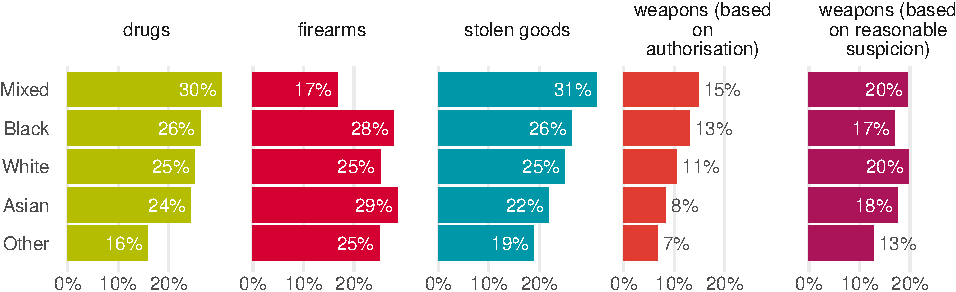
\includegraphics{2020-Q4-bcu_files/figure-latex/chart-outcomes-ethnicity-1} 

}

\caption{Proportion of searches resulting in a formal outcome, January to December 2020}\label{fig:chart-outcomes-ethnicity}
\end{figure}

\hypertarget{where-do-stops-happen}{%
\section{Where do stops happen?}\label{where-do-stops-happen}}

Stop and search is geographically concentrated in some parts of the North West BCU: \textbf{half of searches between January and December 2020 occurred in 11\% of neighbourhoods}. Searches are also concentrated in deprived areas: 58\% of searches took place in neighbourhoods that were more deprived than the BCU average. In particular, 78\% of searches for weapons under section 60 occurred in the most-deprived half of neighbourhoods.

North West BCU had the second lowest number of searches of the 12 Metropolitan Police BCUs. We can identify the areas of the BCU with most searches by dividing it into a grid of equally-sized cells and mapping the density of searches in each grid cell (Figure \ref{fig:chart-map}).

Of the 63 local-authority wards in the North West BCU, the ward with the most searches between January and December 2020 was Harlesden ward in Brent (Table \ref{tab:table-ward}).

\hypertarget{a-note-on-data}{%
\section{A note on data}\label{a-note-on-data}}

This report uses data published by the Home Office at \href{https://data.police.uk/}{data.police.uk} under the \href{https://www.nationalarchives.gov.uk/doc/open-government-licence/version/3/}{Open Government Licence version 3.0} for searches conducted by the Metropolitan Police Service or by British Transport Police at a location in North West BCU.

Search rates are calculated using \href{https://data.london.gov.uk/dataset/ethnic-group-population-projections}{2020 estimates of the London population by age and ethnic group} produced by the Mayor of London. Rates based on residential populations are imperfect because some people being searched in the North West BCU will live in other areas of London or elsewhere, but the local nature of most crime means the majority of people searched in North West BCU are likely to also live there. All ethnicity figures in this report are self-defined ethnicities.

This report is published under a \href{https://creativecommons.org/licenses/by/4.0/}{Creative Commons Attribution Licence version 4.0}, meaning you are free to copy or redistribute this material in any medium or format, and to remix, transform, and build upon this material for any purpose, even commercially, as long as you comply with the licence terms.

Cover photo by \href{https://unsplash.com/photos/eBJrKE3gng8}{Collins Lesulie on Unsplash.com}

\begin{table}

\caption{\label{tab:table-ward}Wards in North West BCU with the highest number of searches, January to December 2020}
\centering
\begin{tabular}[t]{lr}
\toprule
council ward & searches\\
\midrule
1. Harlesden ward, Brent & 1,707\\
2. Greenhill ward, Harrow & 864\\
3. Stonebridge ward, Brent & 830\\
4. Kensal Green ward, Brent & 764\\
5. Dudden Hill ward, Brent & 747\\
6. Wembley Central ward, Brent & 740\\
7. Harrow on the Hill ward, Harrow & 601\\
8. Sudbury ward, Brent & 569\\
9. Mapesbury ward, Brent & 535\\
10. Willesden Green ward, Brent & 494\\
\bottomrule
\end{tabular}
\end{table}

\newgeometry{top = 2cm, inner = 1cm, bottom = 3cm, outer = 1cm}



\begin{figure}[h]

{\centering 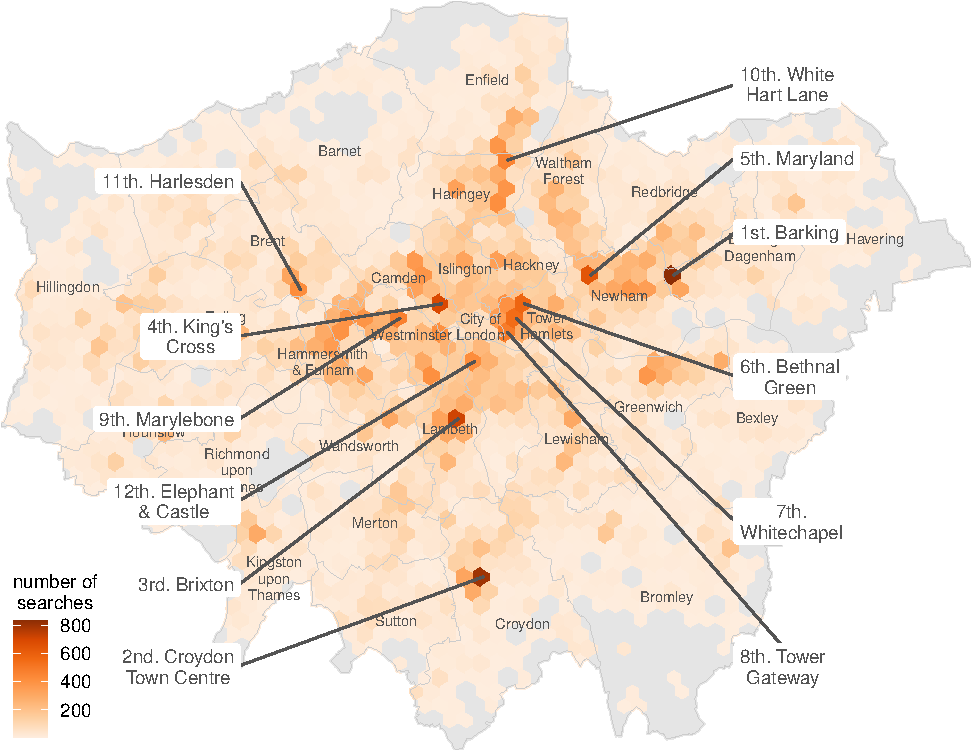
\includegraphics[width=19cm]{2020-Q4-bcu_files/figure-latex/chart-map-1} 

}

\caption{Hotspots of searches, January to December 2020}\label{fig:chart-map}
\end{figure}

\restoregeometry

\end{document}
